\section{Anonymous Protocol}\label{sec-protocol}

\begin{figure}[h]
\begin{center}
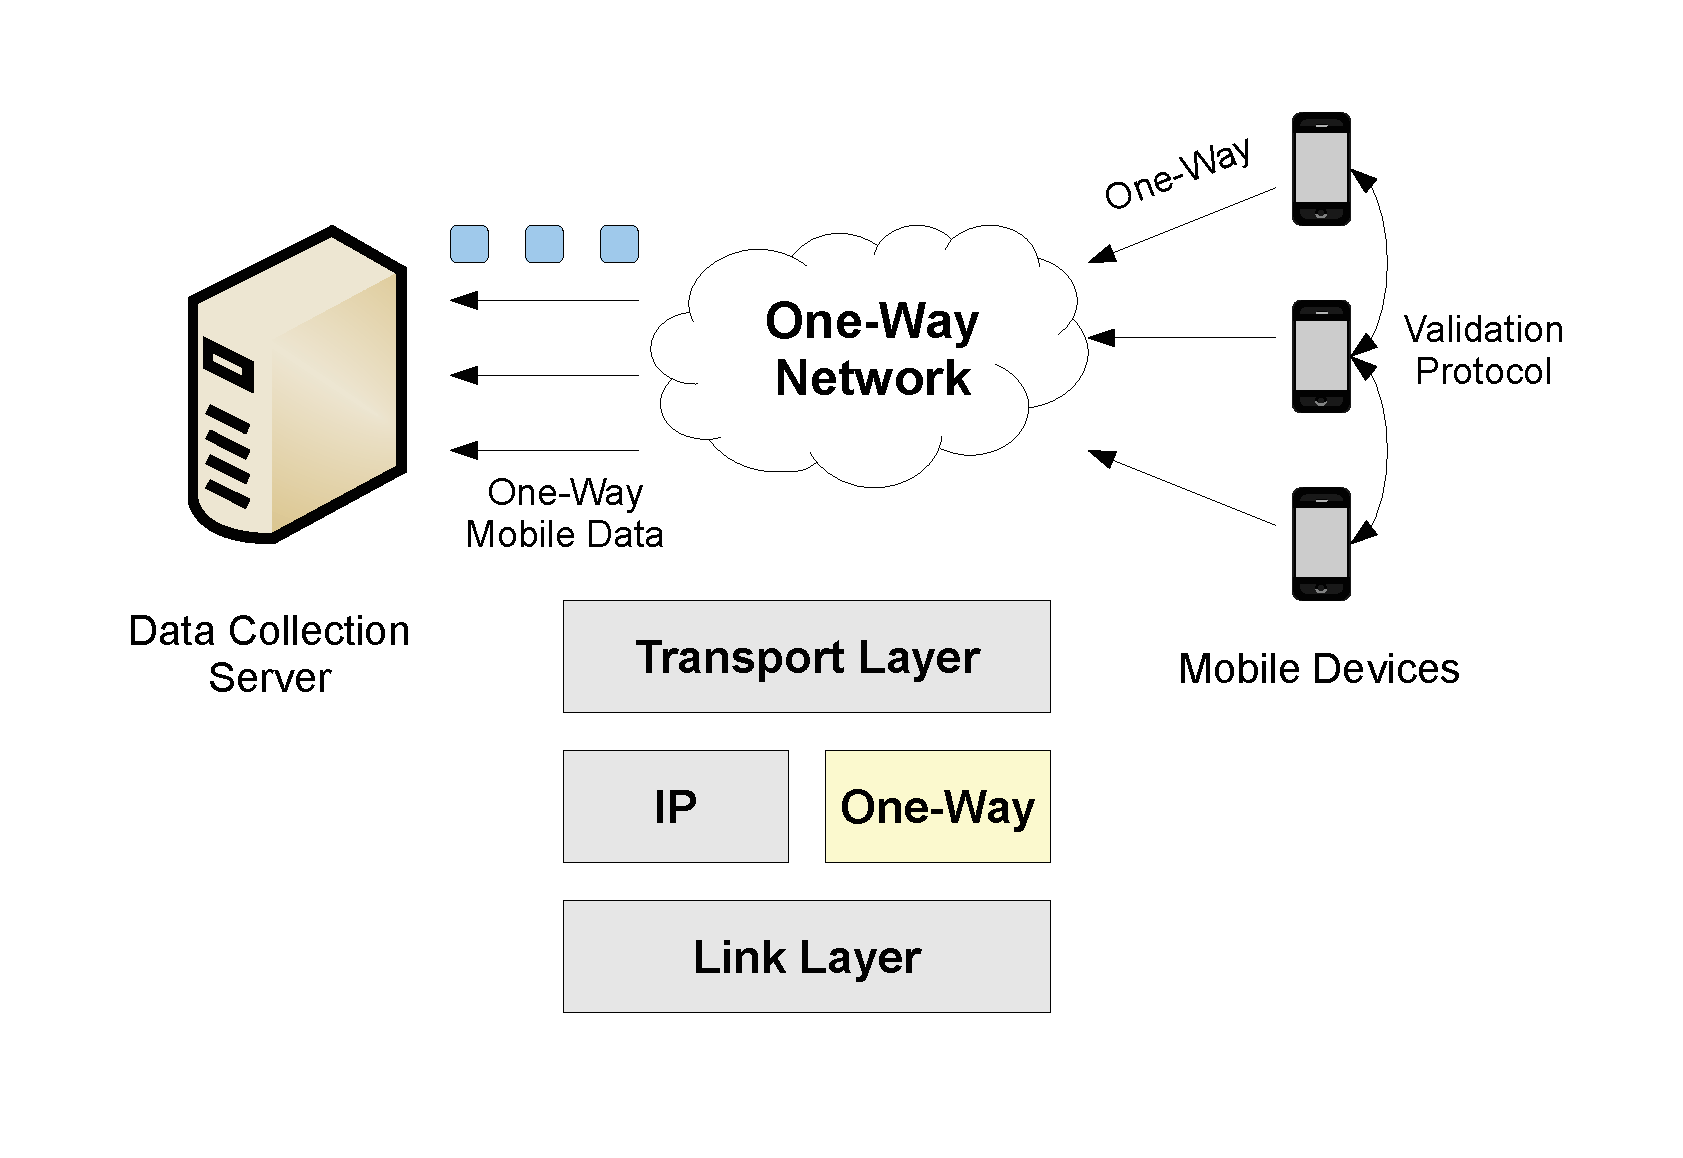
\includegraphics[width=3in]{figure1.eps}
\caption{\small \sl Anonymous Protocol.\label{fig:Stupendous}}
\end{center}
\end{figure}

\subsection{Overview}\label{proto-overview}
In this section, we describe our anonymous One-Way protocol, which completely
removes the ownership and
source information from the data transmitted to the data collection server.
Figure 1 illustrates the concept of the theoretical anonymous One-Way
protocol. One-Way is a packet routing protocol similar to the IP protocol.
Data are transmitted in packets. Each packet contains the address of the destination
host so that the packet can be correctly routed. One major difference between
One-Way protocol and other routing protocol is that, each packet does not
include the routing address of the sender (thus called One-Way). The source
address is intentionally removed so that the receiver of the data does not
know the identity of the sender. In other
words, contractually, the client does not include the source address and the
server will have no access to the source information and thus keeping the
client's identity private.

Our protocol is analogous to sending a parcel through a postal service without
sender's identity and address. An example is sending a hint to the police
pertaining a crime without revealing the sender's identity.

Unlike many other anonymous routing protocols, our protocol does not involve other
peers or mobile devices to transmit the data payload. This is particular helpful
in mobile environment in which bandwidth is limited. Some privacy aware protocols
first transmit the data payload to several mobile peers several times to mask
the identity of the sender before one of the random peers transmit the data to
the server. This puts tremendous bandwidth strain on the peers.

One drawback of a protocol without sender address is that the sender is unable
to get a feedback from the receiver whether a packet has been received (or
lost in transmission). To solve this problem, One-Way utilize a peer-to-peer
approach to verify correct transmission of a packet, much like the way
Crowds\cite{DBLP:journals/tissec/ReiterR98} uses to send data to a server.

Opponents may argue that since the protocol resides on network layer (layer 3),
the source address could still be contained in the lower layer, e.g. the link
layer (layer 2). We argue that the source link address is different for
each hop on the route, and a route could easily contain 20 hops; therefore
the probability of tracing the link layer packet back to the original host is
really low.

\subsection{Anonymous Connection}\label{anonymous_connection}

Before transmitting data to a data collection server (receiver), the
sender makes an anonymous connection request to the server. The purpose
of the connection request is to establish a peer based route on which
acknowledgement of data transmission can be sent.

The sender initiates a connection by constructing an anonymous
connection request packet, $c$. A request packet contains the routing
address (or identification), $A_r$, of the receiver, and a hop count,
$h$. The structure of the request is defined in
Equation~\ref{eq:con_req_format}

\begin{equation}\label{eq:con_req_format}
c = \{I_s, A_r, s_0, h\}, h~\epsilon~\mathbb{N}_{\leq1}
\end{equation}

In the connection request packet, $h$ is a random natural number
denoting the number of peers the request should be forwarded to
before the request is sent to the server.

After the sender has constructed the connection request packet,
it sends the packet to one of its peers running the protocol. When the
peer receives the request, it decrement the hop count $h$ by 1. If
the hop count reaches 0, then the peer sends the request to the server;
else, the peer forwards the request to another one of its peers. Note
a peer does not have to be a pure peer, but a node in the system whose
job is to facilitate communications for user nodes. Each peer in the
route keep track of the peer before and after for each request in order
to maintain the route information. [Address when a peer decline a
connection request].

When the server receives the connection request, it sends back an acceptance
message $a$ to the node from which it receives the connection request.
The acceptance message contains a connection token $I_r$, as well as the
request identifier from the sender, $I_s$. The format of the acceptance
message is defined in Equation~\ref{eq:con_accept_format}

\begin{equation}\label{eq:con_accept_format}
a = \{I_r, I_s\}
\end{equation}

The node that receives the acceptance message from the receiver forwards
the message in reverse to the peer who forwarded the request message.
Each peer in the route keeps the route information based on $I_s$ and
the acceptance messages travels in revers on the same route until the
message reaches the original sender.

[Discussion of the security of this connection approach]

[Briefly describe routing table format and management for example, there
is no activity for a connection for a long time. What should be done?]
\subsection{Payload Transmission}

Payload is the actual data transmitted to the server. In participatory
sensing, this is the data collected by the mobile devices from the
environment and include sensor data, photos, and videos. Payload
transmission does not involve peers since peer-forwarding in wireless
mobile environment is expensive; instead, payloads are transmitted
through the One-Way network, in which the packets only contain receiver
address and identification.

The payload transmission begins when the sender receives the acceptance
message from the server. In addition to the payload $D$, a payload
packet, denoted with $p$, also contains the address of of the receiver
$A_r$, the connection identifier $I_r$, and a sequence number $s$. The
format is defined in Equation~\ref{eq:payload_format}.

\begin{equation}\label{eq:payload_format}
p = \{A_r, I_r, s, D\}
\end{equation}

$I_r$ is the identifier issued by the server received from the connection
acceptance message. The purpose of this identifier is for the server to identify
a particular data transmission. For example, the server could be receiving
several data transmission simultaneously from different client each transmit
a file. The server assigns an identifier $I_r$ to each transmission to
differentiate the packets for the different transmissions. This field is
analogous to the port numbers in transport layers such as TCP and UDP to
multiplex packets for different connections and applications.

The sequence number $s$ in a payload packet identifies individual packets
for a transmission. The sequence numbers provide the order of the packets
and allow the receiver to identify if a packet is lost in the network, or
if packets arrived out of order.

The purpose of the connection establishment step before payload transmission
is to establish a channel in which the mobile client can verify that a packet
has been successfully received by the server. Techniques of reliable data
transfer in unreliable channel is out of scope of this paper. Reliable data
transfer mechanisms employed in TCP\cite{RFC793} and theoretical techniques
such as GO-Back-N and Select Repeat\cite{book:Kurose} can be employed with
our design. When the server wants to send a status of a packet back to
the client, it sends the status message through the peer-to-peer channel
established during connection establishment. In other words, after receiving
a payload packet $p$, the server sends an acknowledgement message, $k$, to the
node from which it received the connection request (also the node to which
it sends the connect acceptance message). Since all nodes on the anonymous route
remembers the previous node based on the connection identifiers, $I_s$ and
$I_r$, each node forwards $k$ to its previous peer until the message
reaches the originator of $p$.

%\begin{figure}[h]
%\begin{center}
%\includegraphics[width=3in]{arch.eps}
%\caption{\small \sl System Architecture.\label{fig:Stupendous}}
%\end{center}
%\end{figure}

\subsection{Node Disconnection and Failure}

When a node can no longer service a route for a connection due to
resource constraint or node shutting down, the disconnecting node (denoted
by $n_d$)
should notify its neighboring nodes of such event so that the interruption
of a connection and of delivering of control messages can be minimized.
In this section, we focus on disconnecting a single connection (as in
the case of resource constraint). If a node wishes to disconnect all
connections it supports (as in the case of node shut down), the $n_d$
performs a disconnection process discussed in this section for each
connection.

There are two scenarios for the $n_d$: the next node is an intermediate node,
and the $n_d$ is the last node in the route ($d$ = $k$).
For the first case in which the the $n_d$ is an intermediate node and the
next node is also an intermediate node, the $n_d$ should simply bridge the
gap and drop off from the route. In this case, the $n_d$ sends the node before
$n_{d-1}$
and after $n_{d+1}$
it a disconnection message containing the identity (the address)
of the two nodes. Once the connection between the two nodes has been
established, $n_d$ can remove the route information for the connection
from its routing table.

In the second case, the $n_d$ is the last node of the route and
communicates directly with the server. In this case, we do not want
just bridge the two nodes $n_{d-1}$ and $n_{d+1}$ since $n_{d-1}$
could be the originator of the data. In order to establish a new route
for the connection, $n_d$ sends a disconnection message to and telling
the server that a new control message route will be constructed for this
connection. $n_d$ also sends a route discovery message to $n_{d-1}$
and telling the node to construct a new route to the server. $n_{d-1}$
follows the same steps described in section~\ref{anonymous_connection}
to establish a new connection the the server.

\begin{algorithm}
\algsetup{linenosize=\small,linenodelimiter=. }
\caption{disconnect($n_d$)} \label{alg:PBSkyline}
\begin{algorithmic}[1]
\IF{$A_d$ = $A_r$}
    \STATE $m_1$ = DisconnectMessage($I_s$, $I_r$)
    \STATE $m_2$ = RediscoveryMessage($I_s$, $I_r$)
    \STATE SendToNode($A_r$, $m_1$)
    \STATE SendToNode($A_{d-1}$, $m_2$)
\ELSE
    \STATE $m_1$ = BridgeMessage($Forward$, $A_{d+1}$, $I_s$, $I_r$)
    \STATE $m_2$ = BridgeMessage($Backward$, $A_{d-1}$, $I_s$, $I_r$)
    \STATE SendToNode($A_{d-1}$, $m_1$)
    \STATE SendToNode($A_{d+1}$, $m_2$)
\ENDIF
\end{algorithmic}
\end{algorithm}

In the event of unforseen failure of a node, such as power or network
failure, the disconnected node $n_d$ is unable to notify its neighbors on
a route before disconnecting. When this happens the first thing that the
sender will notice is that it no longer receives acknowledgement message
of received packet from the server. To test for node failure in the path,
the sender $n_0$ can send a route test message into the route. When a
node $n_m$ receives the test message, it sends an acknowledgement back to
its predecessor $n_{m-1}$ on the route and forwards the test message to
its successor $n_{m+1}$ on the route. If an intermediate node on the route
$n_f$ cannot be contacted or does not acknowledge the test message, then
its predecessor $n_{f-1}$ sends a failure notice backward through the route
to notify the sender a failure has been detected. $n_{f-1}$ uses route
discovery algorithm to discovery a new route from $n_{f-1}$ to the server
and notify the new route has been successfully established. In the case
that there is no failure detected, but the sender still does not receive
acknowledgements from the server, the sender can select to terminate the
data transmission and peer connection.

\subsection{Connection Tear-Down}

After the entire file has been sent to and received by the server, the
sender can choose to tear down the connection so that the nodes can free
the resources used for the connection. To terminate a connection, the
sender injects the termination message identified by $I_s$ and $I_r$ into
the connection. Upon receiving the termination message, a node forwards
the message to its successor and free any resource associated with the
connection. Eventually the termination message reaches the server, and the
server frees the resource, and stores the received file.


\section{Anonymous Protocol Over Existing Protocols}\label{sec-protocol}
The One-Way protocol introduced in the previous section and Figure 1 is only
a theoretical protocol since it would take significant effort and drastic
change to current networking hardware infrastructure to introduce a new layer 3
routing protocol. In this section we modify the One-Way protocol depicted in
Figure 1 slightly so that it utilizes existing networking infrastructures. We
introduce two modifying approaches: tunneling and One-Way over User Datagram
Protocol (UDP).

\subsection{Tunneling}

In tunneling, the network topology is divided into two parts: a private
network that understands the One-Way protocol and the rest of the world that
only understand the IP protocol. The two parts are connected by the tunnel,
a special device, that does the translation between two routing protocols.

\begin{figure}[h]
\begin{center}
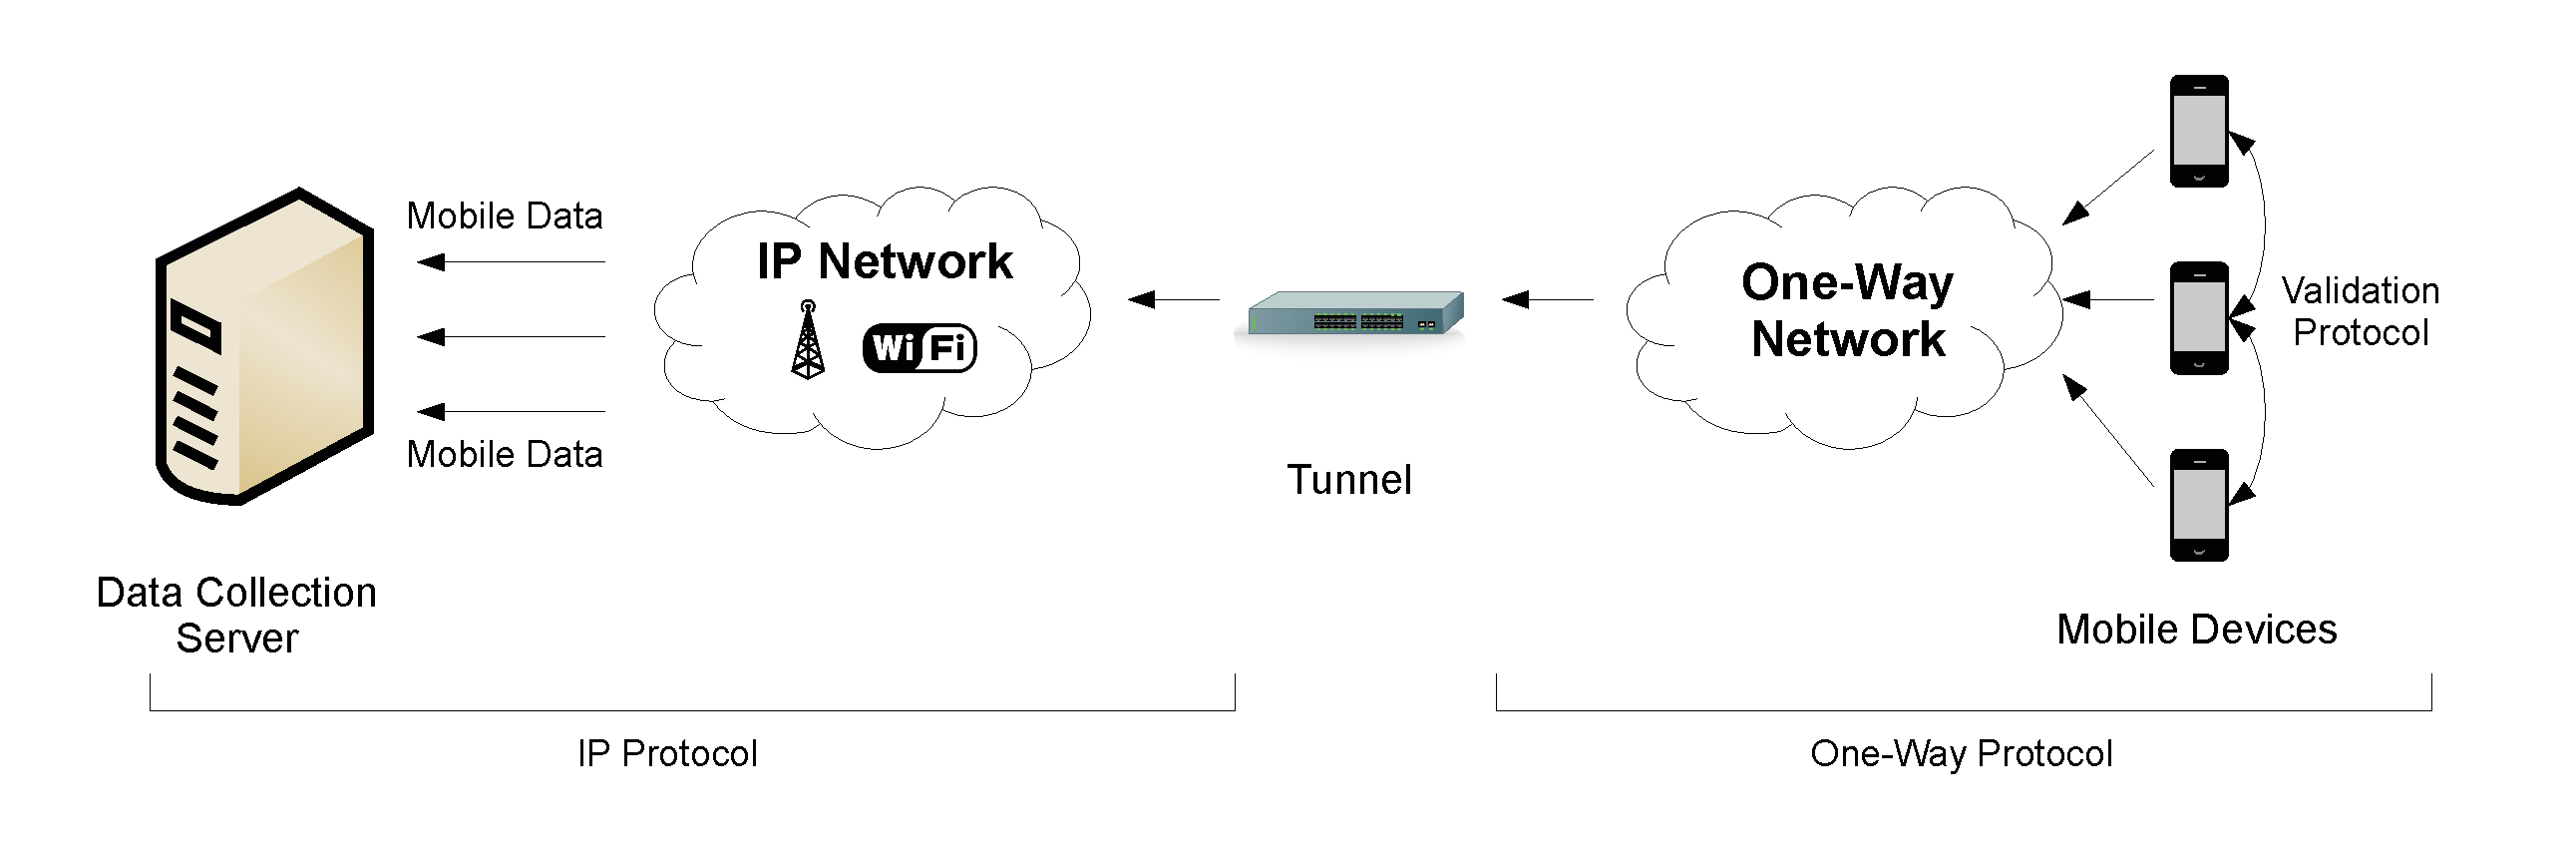
\includegraphics[width=3in]{figure2.eps}
\caption{\small \sl Tunneling.\label{fig:Stupendous}}
\end{center}
\end{figure}

\begin{figure}[h]
\begin{center}
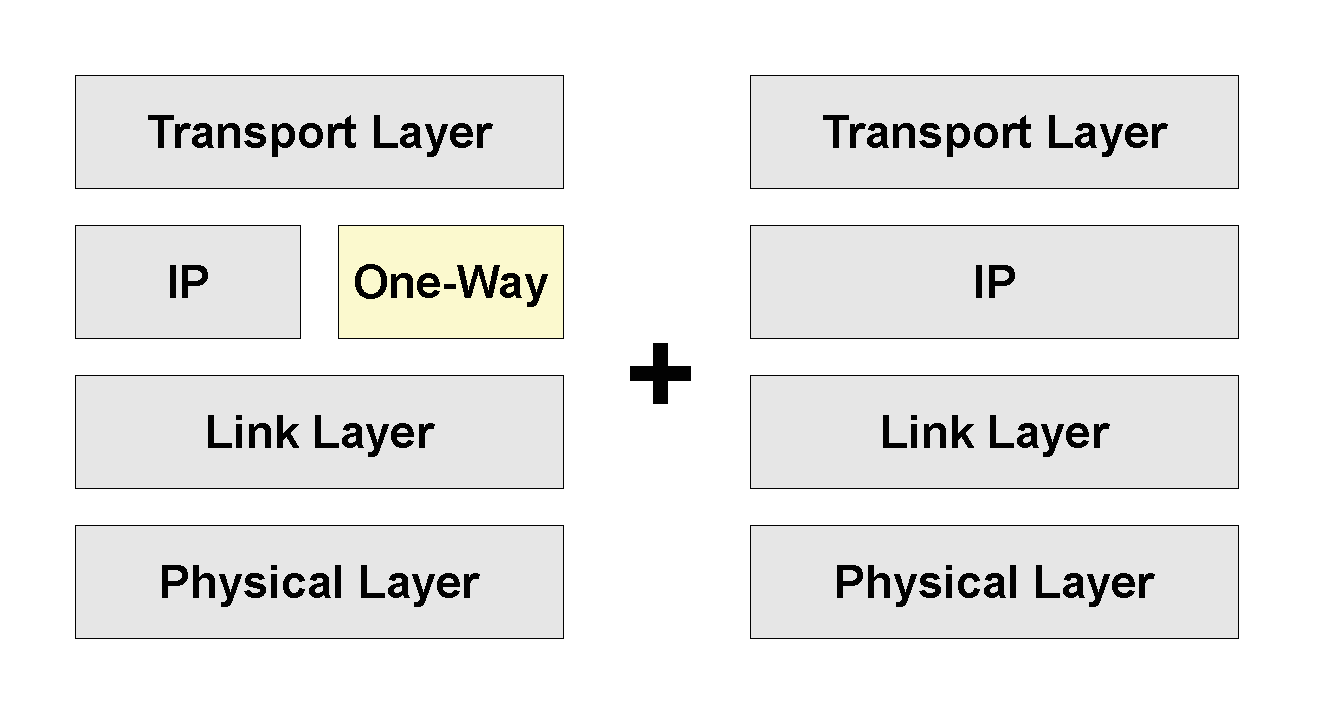
\includegraphics[width=3in]{figure2b.eps}
\caption{\small \sl Tunneling.\label{fig:Stupendous}}
\end{center}
\end{figure}

As illustrated in Figure 2, the tunneling device takes packets from the One-Way
network and forward the
data to the IP network. An important task of the tunneling device is to attach
source IP address to the packets that being forwarded. The device uses it own
IP address as the address of the packets and shields the identity of the mobile
clients. A reason for this tunneling approach is that some internet service
providers (ISP) will block packets without valid source host address. Figure 3
depicts the networking stack configuration of this approach.

Opponent could argument that attacker can still trace the mobile clients to a
specific subnet where the tunneling device resides. We argue that since most of
the clients are highly mobile, and with a number of tunneling device in one
geographic region, the identity of the mobile devices can be protected with high
confidence.

\subsection{Over User Datagram Protocol}
In this approach, we completely do away with a new routing protocol by building
the One-Way protocol as an application layer protocol on top of User Datagram
Protocol (UDP) as illustrated in Figure 4.

\begin{figure}[h]
\begin{center}
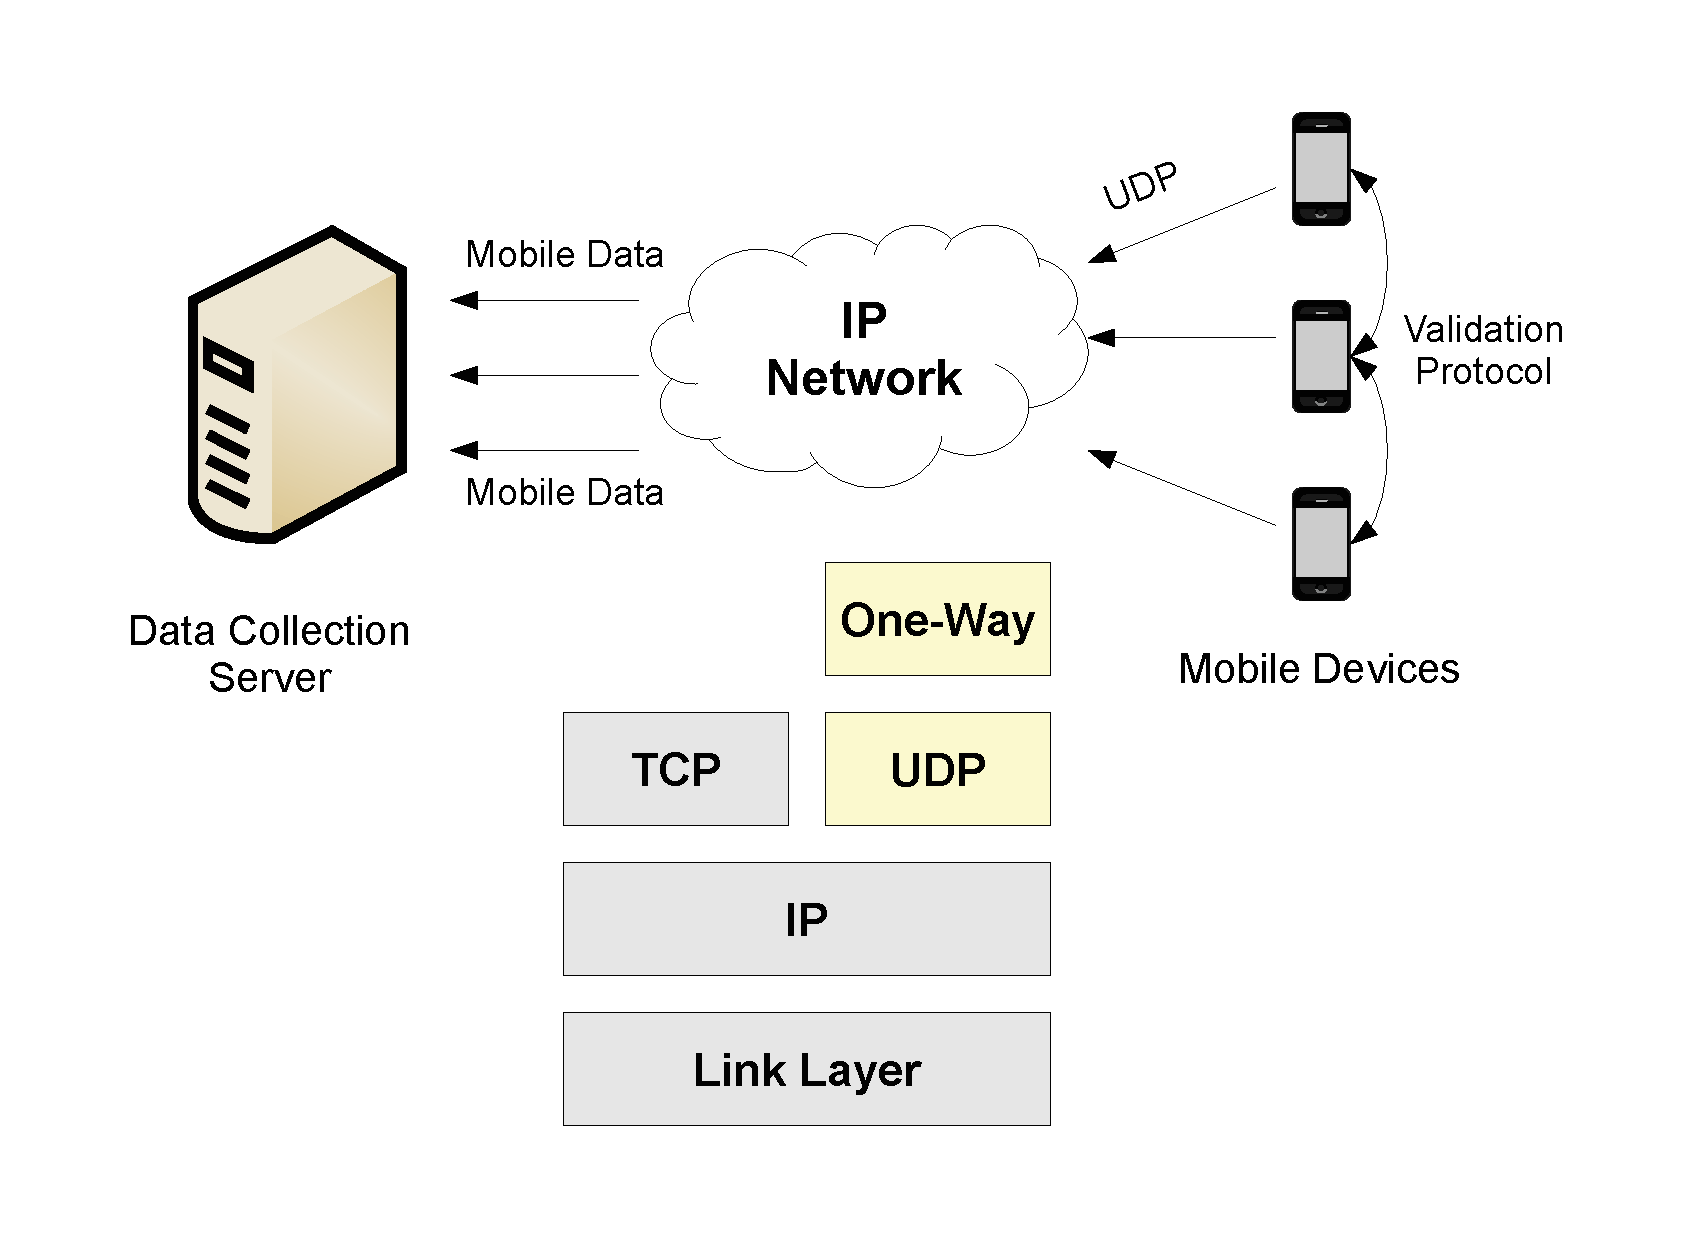
\includegraphics[width=3in]{figure4.eps}
\caption{\small \sl One-Way over UDP.\label{fig:Stupendous}}
\end{center}
\end{figure}

During transmission, the clients divide the data into one or more UDP data packets,
uses arbitrary IP address as the source address -- to protect the identity of the
mobile clients -- and sends the packet into the network.
The reason we use UDP instead of TCP is that since the source IP is arbitrary, TCP
will be unable to establish a connection with the handshaking protocol.

In our experiment, we are able to send IP packets with arbitrary source address into
the network and receive it on the server.

%\section{Validation}
%This section has not been completed.


%\begin{enumerate}
%\item
%The client initiates the K-Nearest-Neighbor Query by evaluating
%$k' = k (r + 1)$ where $r$ is the percentage of replication of original
%dataset. The calculation is done on the client side, since only the data owner
%and the client know the value of $r$. Once found, the clients sends $k'$ to the
%service provider.
%\item
%The service provider finds $k'$ records "surrounding" the location of the
%client based on space encryption Hilbert value. For example, if the Hilbert
%value of the client is $H_c$, then the service provider evaluates the query by
%finding Hilbert values of records in the range $[Hc - K'/2, Hc + K'/2]$.
%Service provider returns the $k'$ records to the client as $R$.
%\item
%Due to Hilbert Space Transformation, locations with the closest Hilbert values
%do not necessary have the closest distance in the original space. To compensate,
%after receiving $R$ from the service provider in step 2, the client finds the
%record, $s^*$, with the largest Hilbert distance from itself, calculate the
%physical distance (or range), $d$, to $s^*$, and performs a range query with
%distance of $d$.
%\end{enumerate}



%\begin{figure}[h]
%\begin{center}
%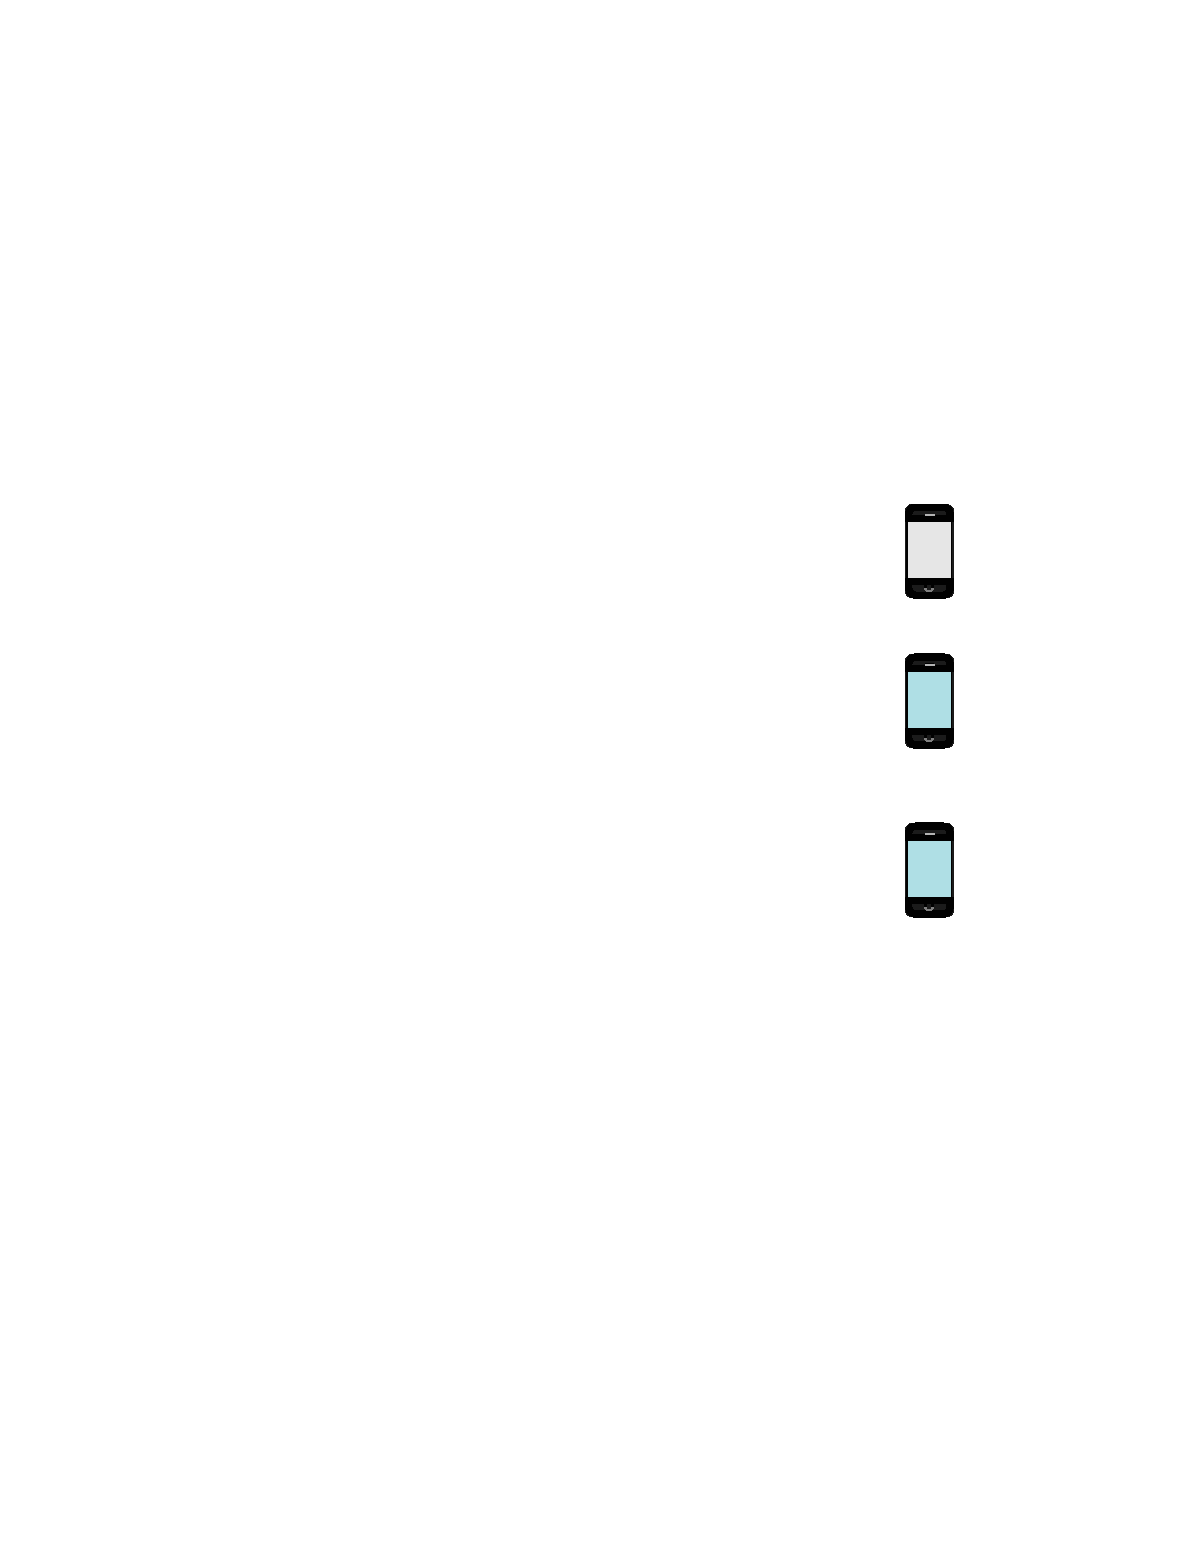
\includegraphics[height=3in]{U1.eps}
%\caption{\small \sl Audit Query Result.\label{fig:Stupendous}}
%\end{center}
%\end{figure}
